\chapter{Metodo alternate direction implicit (ADI)}

\section{La matrice di iterazione in ADI}

Consideriamo il sistema lineare \(\mathbf{A} \mathbf{\phi} = \mathbf{s}\), dove la matrice \(\mathbf{A}\) viene decomposta come:

\[
\mathbf{A} = \mathbf{H} + \mathbf{V} + \mathbf{\Sigma}\ \ ,
\]

dove:
\begin{itemize}
	\item \(\mathbf{H}\): contiene i coefficienti provenienti dalla discretizzazione della parte dipendente da \(x\) dell'operatore Laplaciano;
	\item \(\mathbf{V}\): contiene i coefficienti provenienti dalla discretizzazione della parte dipendente da \(y\) dell'operatore Laplaciano;
	\item \(\mathbf{\Sigma}\): contiene i coefficienti legati all'assorbimento.
\end{itemize}

Ad esempio, per un mezzo omogeneo con griglia uniforme (\(h_{x,i} = h_x\), \(h_{y,j} = h_y\)), l'equazione di diffusione discretizzata è:

\[
\underbrace{-\frac{D}{h_x^2} \phi_{i-1,j} + \frac{2D}{h_x^2} \phi_{i,j} - \frac{D}{h_x^2} \phi_{i+1,j}}_{(\mathbf{H} \mathbf{\phi})_{i,j}}\, -\, \underbrace{\frac{D}{h_y^2} \phi_{i,j-1} + \frac{2D}{h_y^2} \phi_{i,j} - \frac{D}{h_y^2} \phi_{i,j+1}}_{(\mathbf{V} \mathbf{\phi})_{i,j}}\, +\, \underbrace{\Sigma_{a,ij} \phi_{i,j}}_{(\mathbf{\Sigma} \mathbf{\phi})_{i,j}}\ =\ s_{i,j}\ \ . 
\]



\subsection{Procedura iterativa a due passi}

Tale decomposizione della matrice \(\mathbf{A}\) viene utilizzata per impostare una procedura iterativa a due passi. Partendo dall'equazione:

\[
(\mathbf{H} + \mathbf{V} + \mathbf{\Sigma}) \mathbf{\phi} = \mathbf{s}\ \ ,
\]

si riscrive come:

\[
\left(\mathbf{H} + \frac{1}{2} \mathbf{\Sigma}\right) \mathbf{\phi} = -\left(\mathbf{V} + \frac{1}{2} \mathbf{\Sigma}\right) \mathbf{\phi} + \mathbf{s}\ \ . 
\]

Un parametro di rilassamento \(\omega\) viene introdotto sommando a entrambi i membri dell'equazione sopra la stessa quantità \(\omega \mathbf{\phi}\), ottenendo:

\[
\left(\mathbf{H} + \frac{1}{2} \mathbf{\Sigma} + \omega \mathbf{I}\right) \mathbf{\phi} = \left(\omega \mathbf{I} - \mathbf{V} - \frac{1}{2} \mathbf{\Sigma}\right) \mathbf{\phi} + \mathbf{s}\ \ . 
\]

In modo equivalente, si può scrivere:

\[
\left(\mathbf{V} + \frac{1}{2} \mathbf{\Sigma} + \omega \mathbf{I}\right) \mathbf{\phi} = \left(\omega \mathbf{I} - \mathbf{H} - \frac{1}{2} \mathbf{\Sigma}\right) \mathbf{\phi} + \mathbf{s}\ \ . 
\]



\subsection{Schema iterativo}

Lo schema iterativo che ne segue è:

\[ \begin{aligned}
& \text{$1^{\circ}$ passo:} \quad \left(\mathbf{H} + \frac{1}{2} \mathbf{\Sigma} + \omega \mathbf{I}\right) \mathbf{\phi}^{\left(m+\frac{1}{2}\right)} = \left(\omega \mathbf{I} - \mathbf{V} - \frac{1}{2} \mathbf{\Sigma}\right) \mathbf{\phi}^{(m)} + \mathbf{s}\ \ ,  \\
& \text{$2^{\circ}$ passo:} \quad \left(\mathbf{V} + \frac{1}{2} \mathbf{\Sigma} + \omega \mathbf{I}\right) \mathbf{\phi}^{(m+1)} = \left(\omega \mathbf{I} - \mathbf{H} - \frac{1}{2} \mathbf{\Sigma}\right) \mathbf{\phi}^{\left(m+\frac{1}{2}\right)} + \mathbf{s}\ \ . \end{aligned}\]

Ogni iterazione \(m\) è quindi composta da due semi-iterazioni, date dalle equazioni precedenti.
Una velocità di convergenza migliore si ottiene se il parametro \(\omega\) viene cambiato ciclicamente, adottando lo schema:

\[
\begin{aligned}
	& \left(\mathbf{H} + \frac{1}{2} \mathbf{\Sigma} + \omega_m \mathbf{I}\right) \mathbf{\phi}^{\left(m+\frac{1}{2}\right)} = \left(\omega_m \mathbf{I} - \mathbf{V} - \frac{1}{2} \mathbf{\Sigma}\right) \mathbf{\phi}^{(m)} + \mathbf{s}\ , \\
	& \left(\mathbf{V} + \frac{1}{2} \mathbf{\Sigma} + \omega_m \mathbf{I}\right) \mathbf{\phi}^{(m+1)} = \left(\omega_m \mathbf{I} - \mathbf{H} - \frac{1}{2} \mathbf{\Sigma}\right) \mathbf{\phi}^{\left(m+\frac{1}{2}\right)} + \mathbf{s}\ \ . 
\end{aligned}
\]



\subsection{Struttura delle matrici}

In base alle relazioni iniziali, ogni semi-iterazione ha la forma di un'equazione a tre punti, sebbene solo la prima sia tridiagonale.
Considerando il sistema di $3\times 3$ nodi mostrato in figura, la decomposizione adottata produce matrici con la seguente struttura:

\[
\mathbf{A} = \mathbf{H} + \mathbf{V} + \mathbf{\Sigma}
\]

\[\begin{aligned}
\left[
\begin{array}{c c c c c c c c c}
	\times & \times & 0 & \times & 0 & 0 & 0 & 0 & 0 \\
	\times & \times & \times & 0 & \times & 0 & 0 & 0 & 0 \\
	0 & \times & \times & 0 & 0 & \times & 0 & 0 & 0 \\
	\times & 0 & 0 & \times & \times & 0 & \times & 0 & 0 \\
	0 & \times & 0 & \times & \times & \times & 0 & \times & 0 \\
	0 & 0 & \times & 0 & \times & \times & 0 & 0 & \times \\
	0 & 0 & 0 & \times & 0 & 0 & \times & \times & 0 \\
	0 & 0 & 0 & 0 & \times & 0 & \times & \times & \times \\
	0 & 0 & 0 & 0 & 0 & \times & 0 & \times & \times
\end{array}
\right]\ &=\
\left[\underset{\underset{(\text{tridiagonal})}{\mathbf{H} + \frac{1}{2}\mathbf{\Sigma}}}{\begin{array}{c c c c c c c c c}
	\times & \times & 0 & 0 & 0 & 0 & 0 & 0 & 0 \\
	\times & \times & \times & 0 & 0 & 0 & 0 & 0 & 0 \\
	0 & \times & \times & 0 & 0 & 0 & 0 & 0 & 0 \\
	0 & 0 & 0 & \times & \times & 0 & 0 & 0 & 0 \\
	0 & 0 & 0 & \times & \times & \times & 0 & 0 & 0 \\
	0 & 0 & 0 & 0 & \times & \times & 0 & 0 & 0 \\
	0 & 0 & 0 & 0 & 0 & 0 & \times & \times & 0 \\
	0 & 0 & 0 & 0 & 0 & 0 & \times & \times & \times \\
	0 & 0 & 0 & 0 & 0 & 0 & 0 & \times & \times
\end{array}
}\right]\\
&\, +\, 
\left[
\underset{\underset{(\text{Band matrix})}{\mathbf{V} + \frac{1}{2}\mathbf{\Sigma}}}{\begin{array}{c c c c c c c c c}
		\times & 0 & 0 & \times & 0 & 0 & 0 & 0 & 0 \\
		0 & \times & 0 & 0 & \times & 0 & 0 & 0 & 0 \\
		0 & 0 & \times & 0 & 0 & \times & 0 & 0 & 0 \\
		\times & 0 & 0 & \times & 0 & 0 & \times & 0 & 0 \\
		0 & \times & 0 & 0 & \times & 0 & 0 & \times & 0 \\
		0 & 0 & \times & 0 & 0 & \times & 0 & 0 & \times \\
		0 & 0 & 0 & \times & 0 & 0 & \times & 0 & 0 \\
		0 & 0 & 0 & 0 & \times & 0 & 0 & \times & 0 \\
		0 & 0 & 0 & 0 & 0 & \times & 0 & 0 & \times
	\end{array}
	} 
\right]\end{aligned}
\]



L'aggiunta della matrice \(\omega_m \mathbf{I}\) non modifica la struttura delle matrici a destra dell'uguale.
Pertanto, \(\mathbf{H} + \frac{1}{2} \mathbf{\Sigma} + \omega_m \mathbf{I}\) è tridiagonale e può essere risolta con l'algoritmo di Thomas nella prima semi-iterazione.

La matrice \(\mathbf{V} + \frac{1}{2} \mathbf{\Sigma} + \omega_m \mathbf{I}\) è invece una matrice a banda. Tuttavia, è possibile trovare una matrice di permutazione \(\mathbf{P}\) tale che:

\[
\mathbf{P} \left(\mathbf{V} + \frac{1}{2} \mathbf{\Sigma} + \omega_m \mathbf{I}\right) \mathbf{P}^T \quad \Rightarrow \quad \text{è tridiagonale},
\]

rendendo possibile l'uso dell'algoritmo di Thomas anche per la seconda semi-iterazione.

\begin{figure}[H]
	\centering
	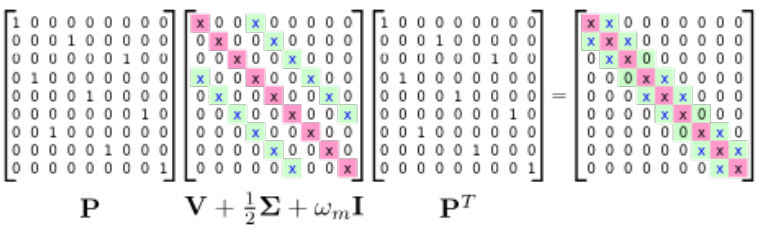
\includegraphics[width=10cm]{img/exampleADI.png}
	\label{esempio ADI}
	\caption{esempio}
\end{figure}

%
%
\subsection{Risoluzione delle semi-iterazioni}

Dall'equazione trovata per lo schema iterativo si ottiene:

\[\begin{aligned}
\mathbf{\phi}^{\left(m+\frac{1}{2}\right)}&= \left(\mathbf{H} + \frac{1}{2} \mathbf{\Sigma} + \omega_m \mathbf{I}\right)^{-1} \left[ \left(\omega_m \mathbf{I} - \mathbf{V} - \frac{1}{2} \mathbf{\Sigma}\right) \mathbf{\phi}^{(m)} + \mathbf{s} \right]\ =\\
&=\ \left(\mathbf{H} + \frac{1}{2} \mathbf{\Sigma} + \omega_m \mathbf{I}\right)^{-1} \left(\omega_m \mathbf{I} - \mathbf{V} - \frac{1}{2} \mathbf{\Sigma}\right) \mathbf{\phi}^{(m)} + \hat{\mathbf{s}}\ \ ,\end{aligned}
\]

dove

\[
\hat{\mathbf{s}} = \left(\mathbf{H} + \frac{1}{2} \mathbf{\Sigma} + \omega_m \mathbf{I}\right)^{-1} \mathbf{s}\ \ .
\]

Analogamente, sostituendo \(\mathbf{\phi}^{\left(m+\frac{1}{2}\right)}\), si ottiene la matrice di iterazione corrispondente all'insieme delle due semi-iterazioni.



\subsection{Matrice di iterazione del metodo ADI}

\[
\begin{aligned}
	\mathbf{\phi}^{(m+1)} &= \left(\mathbf{V} + \frac{1}{2} \mathbf{\Sigma} + \omega_m \mathbf{I}\right)^{-1} \left(\omega_m \mathbf{I} - \mathbf{H} - \frac{1}{2} \mathbf{\Sigma}\right) \mathbf{\phi}^{\left(m+\frac{1}{2}\right)} + \tilde{\mathbf{s}}\ = \\
	&= \left(\mathbf{V} + \frac{1}{2} \mathbf{\Sigma} + \omega_m \mathbf{I}\right)^{-1} \left(\omega_m \mathbf{I} - \mathbf{H} - \frac{1}{2} \mathbf{\Sigma}\right) \left[ \left(\mathbf{H} + \frac{1}{2} \mathbf{\Sigma} + \omega_m \mathbf{I}\right)^{-1} \right. \\
	&\quad \left. \cdot \left(\omega_m \mathbf{I} - \mathbf{V} - \frac{1}{2} \mathbf{\Sigma}\right) \mathbf{\phi}^{(m)} + \hat{\mathbf{s}} \right] + \tilde{\mathbf{s}} \\
	&= \mathbf{J}_{\omega} \mathbf{\phi}^{(m)} + \mathbf{Q},
\end{aligned}
\]

dove la matrice di iterazione \(\mathbf{J}_{\omega}\) è definita come:

\[
\mathbf{J}_{\omega} = \left(\mathbf{V} + \frac{1}{2} \mathbf{\Sigma} + \omega_m \mathbf{I}\right)^{-1} \left(\omega_m \mathbf{I} - \mathbf{H} - \frac{1}{2} \mathbf{\Sigma}\right) \cdot \left(\mathbf{H} + \frac{1}{2} \mathbf{\Sigma} + \omega_m \mathbf{I}\right)^{-1} \left(\omega_m \mathbf{I} - \mathbf{V} - \frac{1}{2} \mathbf{\Sigma}\right).
\]


%
%
%
\subsection{Convergenza del metodo ADI}

È possibile dimostrare che, per qualsiasi \(\omega > 0\), il raggio spettrale di \(\mathbf{J}_{\omega}\) è minore di 1.
La dimostrazione parte dalla considerazione che, se ovunque è \(\Sigma_a > 0\) (come effettivamente accade), le matrici:

\[
\mathbf{H} + \frac{1}{2} \mathbf{\Sigma} \qquad \text{e} \qquad \mathbf{V} + \frac{1}{2} \mathbf{\Sigma}
\]

sono simmetriche e definite positive (SPD). Pertanto, i loro autovalori sono reali e positivi, e lo stesso vale per tutti gli autovalori \(\lambda_i\) di \(\mathbf{J}_{\omega}\).

Si dimostra quindi che, se \(\omega_m > 0\), tutti gli autovalori \(\lambda_i\) di \(\mathbf{J}_{\omega}\) sono minori di 1, cioè:

\[
0 < \lambda_i < 1 \quad \forall i.
\]

Di conseguenza, \underline{\(\left| \lambda_i \right| < 1\) per ogni \(i\), garantendo la convergenza del metodo ADI}.

%
%
\section{ADI per problemi separabili}

Consideriamo l'equazione di diffusione stazionaria 2D scritta nella forma:

\[
\nabla^2 \phi(\mathbf{r}) + B^2 \phi(\mathbf{r}) = 0 
\quad \Rightarrow \quad 
\frac{\partial^2 \phi(\mathbf{r})}{\partial x^2} + \frac{\partial^2 \phi(\mathbf{r})}{\partial y^2} + B^2 \phi(\mathbf{r}) = 0\ \ . 
\]

Analizziamo un problema separabile, in cui il flusso può essere espresso come prodotto di due funzioni di una sola variabile: $\phi(x, y)\ =\ X(x)\ Y(y)$. Sostituendo nell'equazione di diffusione, si ottiene:

\[
\frac{1}{X}\, \frac{\partial^2 X}{\partial x^2}\ +\ \frac{1}{Y}\, \frac{\partial^2 Y}{\partial y^2}\, +\, B^2\ =\ 0\ \ .
\]

Poiché \(x\) e \(y\) sono variabili indipendenti, i primi due termini dell'equazione devono essere costanti. Pertanto:

\[
\frac{1}{X_k}\, \frac{d^2 X_k}{dx^2}\ =\ -\,B_k^2\ \ , 
\]

\[
\frac{1}{Y_l}\, \frac{d^2 Y_l}{dy^2}\ =\ -B\,_l^2\ \ , 
\]

con la condizione: $B_k^2\ +\ B_l^2\ =\ B^2$ .

Le due equazioni sopra sono equazioni agli autovalori: \(X_k\), \(B_k^2\) e \(Y_l\), \(B_l^2\) rappresentano, rispettivamente, gli autofunzioni e gli autovalori corrispondenti (\(k, l = 1, \dots, \infty\)).

La soluzione generale \(\phi_{k,l} = X_k\, Y_l\) è quindi un'autofunzione di entrambe, ma con autovalori diversi:

\[
\frac{\partial^2 \phi_{k,l}}{\partial x^2} = -B_k^2 \phi_{k,l} \quad \text{e} \quad \frac{\partial^2 \phi_{k,l}}{\partial y^2} = -B_l^2 \phi_{k,l}. 
\]

Lo stesso vale per la versione discretizzata dell'equazione di diffusione, cioè per le matrici \(\mathbf{H}\) e \(\mathbf{V}\), nonché per \(\mathbf{H} + \frac{1}{2}\mathbf{\Sigma}\) e \(\mathbf{V} + \frac{1}{2}\mathbf{\Sigma}\), che condividono gli stessi autovettori \(\phi_{k,l}\) ma con autovalori diversi:

\[
\left(\mathbf{H} + \frac{1}{2}\mathbf{\Sigma}\right) \phi_{k,l} = \lambda_k \phi_{k,l}, 
\]

\[
\left(\mathbf{V} + \frac{1}{2}\mathbf{\Sigma}\right) \phi_{k,l} = \mu_l \phi_{k,l}, \quad (k=1,\dots,n_x; \ l=1,\dots,n_y) 
\]

dove \(n_x\) e \(n_y\) sono il numero di nodi nelle direzioni \(x\) e \(y\).
Gli autovalori \(\lambda_k\) e \(\mu_l\) hanno, rispettivamente, molteplicità \(n_y\) e \(n_x\) (ad esempio, gli \(n_y\) autovettori \(\phi_{1,l}\) (\(l=1,\dots,n_y\)) condividono lo stesso autovalore \(\lambda_1\)).
Il numero totale di autovalori è \(n_x \cdot n_y\).


\subsection{Raggio spettrale della matrice di iterazione \(\mathbf{J}_{\omega}\)}

Considerando la matrice di iterazione \(\mathbf{J}_{\omega}\), le quattro matrici che la compongono hanno tutte lo stesso autovettore \(\phi_{k,l}\). Pertanto:

\[
\mathbf{J}_{\omega} \phi_{k,l}\ =\ \frac{\omega_m - \lambda_k}{\omega_m + \lambda_k} \frac{\omega_m - \mu_l}{\omega_m + \mu_l}\, \phi_{k,l}\ \ , 
\]

e il suo raggio spettrale è dato da:

\[
\rho_{\mathbf{J}_{\omega}} = \max_{k,l} \left| \frac{\omega_m - \lambda_k}{\omega_m + \lambda_k} \frac{\omega_m - \mu_l}{\omega_m + \mu_l} \right|. \tag{19}
\]

Poiché \(\lambda_k, \mu_l > 0\) per ogni \((k,l)\), si ha:

\[
\omega_m > 0 \quad \Rightarrow \quad \rho_{\mathbf{J}_{\omega}} < 1.
\]

\subsection{Scelta ottimale dei parametri \(\omega\)}

Immaginiamo ora di utilizzare due valori distinti del parametro \(\omega\), ad esempio \(\omega_1\) e \(\omega_2\), e di eseguire una prima iterazione completa (cioè due semi-iterazioni) con \(\omega = \omega_1\) e poi una seconda con \(\omega = \omega_2\).
La matrice di iterazione associata a questa iterazione composta è quindi uguale al prodotto \(\mathbf{J}_{\omega_2},\, \mathbf{J}_{\omega_1}\), e si ha:

\[
\mathbf{J}_{\omega_2}\, \mathbf{J}_{\omega_1}\, \phi_{k,l}\ =\ \frac{\omega_2 - \lambda_k}{\omega_2 + \lambda_k} \frac{\omega_2 - \mu_l}{\omega_2 + \mu_l} \frac{\omega_1 - \lambda_k}{\omega_1 + \lambda_k} \frac{\omega_1 - \mu_l}{\omega_1 + \mu_l}\, \phi_{k,l}\ \ ,
\]

quindi:

\[
\rho_{\mathbf{J}_{\omega_2} \mathbf{J}_{\omega_1}}\ =\ \max_{k,l} \left| \frac{\omega_2 - \lambda_k}{\omega_2 + \lambda_k} \frac{\omega_2 - \mu_l}{\omega_2 + \mu_l} \frac{\omega_1 - \lambda_k}{\omega_1 + \lambda_k} \frac{\omega_1 - \mu_l}{\omega_1 + \mu_l} \right|\ \ .
\]

Per una iterazione composta da \(p\) iterazioni complete, si ha:

\[
\rho_{\mathbf{J}_{\omega_p} \cdots \mathbf{J}_{\omega_1}} = \max_{k,l} \left| \frac{\omega_p - \lambda_k}{\omega_p + \lambda_k} \frac{\omega_p - \mu_l}{\omega_p + \mu_l} \cdots \frac{\omega_2 - \lambda_k}{\omega_2 + \lambda_k} \frac{\omega_2 - \mu_l}{\omega_2 + \mu_l} \frac{\omega_1 - \lambda_k}{\omega_1 + \lambda_k} \frac{\omega_1 - \mu_l}{\omega_1 + \mu_l} \right|. \tag{21}
\]

Se \(p\) è pari al numero \(n_x\) di autovalori distinti di \(\mathbf{H} + \frac{1}{2}\mathbf{\Sigma}\) e i parametri \(\omega\) sono scelti in modo che \(\omega_1 = \lambda_1, \omega_2 = \lambda_2, \dots, \omega_{n_x} = \lambda_{n_x}\), il raggio spettrale \(\rho_{\mathbf{J}_{\omega_p} \cdots \mathbf{J}_{\omega_1}}\) è uguale a zero.
Infatti, nell'ultima equazione, per ogni coppia \((k,l)\) esiste sempre un fattore nullo.

In queste condizioni, il processo iterativo raggiunge la soluzione esatta in un numero finito di iterazioni.



\subsubsection{Esempio con sistema 2x2 nodi}

Consideriamo un sistema di \(2 \times 2\) nodi (\(n_x = n_y = 2\)) e poniamo \(p = n_x = 2\). Gli autovalori \(\delta_i\) della matrice di iterazione \(\mathbf{J}_{\omega_2},\, \mathbf{J}_{\omega_1}\) sono:

\[
\begin{aligned}
	\delta_1 &= \frac{\omega_2 - \lambda_1}{\omega_2 + \lambda_1} \frac{\omega_2 - \mu_1}{\omega_2 + \mu_1} \frac{\omega_1 - \lambda_1}{\omega_1 + \lambda_1} \frac{\omega_1 - \mu_1}{\omega_1 + \mu_1}, \\
	\delta_2 &= \frac{\omega_2 - \lambda_1}{\omega_2 + \lambda_1} \frac{\omega_2 - \mu_2}{\omega_2 + \mu_2} \frac{\omega_1 - \lambda_1}{\omega_1 + \lambda_1} \frac{\omega_1 - \mu_2}{\omega_1 + \mu_2}, \\
	\delta_3 &= \frac{\omega_2 - \lambda_2}{\omega_2 + \lambda_2} \frac{\omega_2 - \mu_1}{\omega_2 + \mu_1} \frac{\omega_1 - \lambda_2}{\omega_1 + \lambda_2} \frac{\omega_1 - \mu_1}{\omega_1 + \mu_1}, \\
	\delta_4 &= \frac{\omega_2 - \lambda_2}{\omega_2 + \lambda_2} \frac{\omega_2 - \mu_2}{\omega_2 + \mu_2} \frac{\omega_1 - \lambda_2}{\omega_1 + \lambda_2} \frac{\omega_1 - \mu_2}{\omega_1 + \mu_2}.
\end{aligned}
\]

Se scegliamo \(\omega_1 = \lambda_1\) e \(\omega_2 = \lambda_2\), si ottiene:

\[
\delta_1 = \delta_2 = \delta_3 = \delta_4 = 0 \quad \Rightarrow \quad \rho_{\mathbf{J}_{\omega_2} \mathbf{J}_{\omega_1}} = 0.
\]


\subsubsection{Stima dell'intervallo \([\alpha, \beta]\) per gli autovalori}

Tuttavia, la conoscenza di tutti gli autovalori della matrice \(\mathbf{H} + \frac{1}{2}\mathbf \Sigma\) (o \(\mathbf{V} + \frac{1}{2}\mathbf\Sigma\)) è spesso un compito molto difficile.
Inoltre, essendo il numero di autovalori molto elevato, potrebbe non essere conveniente eseguire anche una singola iterazione composta.

L'idea è quindi di stimare un intervallo \([\alpha, \beta]\) che contenga tutti gli autovalori delle suddette matrici, cioè tale che: $\alpha \leq \lambda_k, \mu_l \leq \beta \quad \forall\ k, l$.



\subsubsection{Minimizzazione del raggio spettrale}

Dall'equazione del raggio spettrale possiamo scrivere:

\[
\begin{aligned}
	\rho_{\mathbf{J}_{\omega_p} \cdots \mathbf{J}_{\omega_1}} &= \max_k \left( \left| \frac{\omega_p - \lambda_k}{\omega_p + \lambda_k} \cdots \frac{\omega_2 - \lambda_k}{\omega_2 + \lambda_k} \frac{\omega_1 - \lambda_k}{\omega_1 + \lambda_k} \right| \right) \\
	&\quad \cdot \max_l \left( \left| \frac{\omega_p - \mu_l}{\omega_p + \mu_l} \cdots \frac{\omega_2 - \mu_l}{\omega_2 + \mu_l} \frac{\omega_1 - \mu_l}{\omega_1 + \mu_l} \right| \right) \\
	&\leq \left[ \max_{\alpha \leq x \leq \beta} \left| \frac{\omega_p - x}{\omega_p + x} \cdots \frac{\omega_2 - x}{\omega_2 + x} \frac{\omega_1 - x}{\omega_1 + x} \right| \right]^2\ \ . 
\end{aligned}
\]

Poiché \(\alpha \leq x \leq \beta\), se \(x\) è tale da restituire il valore massimo, i due termini possono, al massimo, uguagliarlo, giustificando così l'ultima disuguaglianza.

Il problema si riduce quindi a minimizzare il contenuto tra parentesi quadrate, cioè:

\[
\min_{\omega_p, \dots, \omega_2, \omega_1} \max_{\alpha \leq x \leq \beta} \left| \frac{\omega_p - x}{\omega_p + x} \cdots \frac{\omega_2 - x}{\omega_2 + x} \frac{\omega_1 - x}{\omega_1 + x} \right|. \tag{24}
\]


\section{Considerazioni finali}

- Senza l'uso di un parametro di rilassamento \(\omega\), il metodo ADI è generalmente meno performante del metodo LOR. Dalle equazioni di semi-iterazione si osserva che ogni semi-iterazione si basa sui flussi del passo precedente, anche se sarebbero disponibili valori aggiornati.

- Per problemi non separabili, non esiste una teoria rigorosa per la selezione dei parametri \(\omega\).

- Pertanto, il metodo ADI offre prestazioni ottimali per problemi separabili, mentre può essere molto meno efficiente per problemi non separabili.

- Per un problema quasi separabile, è possibile utilizzare il problema separabile più vicino come "problema modello" per calcolare i parametri \(\omega\). In generale, tali parametri forniscono buone prestazioni anche per problemi quasi separabili.